\section{Method}
\label{sec:model}

\subsection{Dataset}
\label{subsec:dat}
We collected 13,238,863 tweets from August 10, 2014 to August 27, 2014 mentioning Ferguson using the Twitter Streaming API. Among them 92,184 are geo-tagged, which takes about 0.70\% of all. We use geo-tagged tweets instead of all tweets so that we could separate tweets in \stlouis from those are not. We use 2014 TIGER/Lines Shapefile to identify the locations of tweets according to coordinates.\footnote{\url{https://www.census.gov/geo/maps-data/data/tiger-line.html}}

News are crawled by the links published by news account on Twitter. We selected 108 media accounts from Twitter, for example ``Washington Post", ``NBC News" and ``ABC7News", collected all the tweets they published during the Ferguson event, and extracted news reports from the links they published. In total, there are 1,338 news covering from August 11 to 27.

Same standard preprocessing procedure is applied to news and Twitter corpora, such as tokenization, POS tagging, lemmatization, bigrams detection, stop words, low frequency words and too high frequency words removal. After preprocessing and removing empty documents, there are 1,275 news documents and 81,553 Twitter documents, as well as a vocabulary with 1,132 words.

%However, we use different tools for the two corpora: OpenNLP package~\cite{baldridge2005opennlp} for news corpus and Tweet NLP package~\cite{owoputi2013improved} for Twitter corpus.

\subsection{Single Topic LDA Model}

We propose \stlda to deal with short documents like tweets and long documents like news simultaneously. The intuition is that short documents are unlikely to be related to multiple topics. Instead, one short document is usually talking about a single topic and all its words are generated from this topic. Meanwhile, long documents still follow conventional LDA assumptions: each document contains a mixture of topics. Specifically, the generative process of tweets and news is defined as

\begin{enumerate}
\item For each topic $k \in \{1, \ldots, K\}$
    \begin{enumerate}
    \item Draw word distribution $\bm{\phi_k} \sim \mathrm{Dir}(\beta)$
    \end{enumerate}
\item For each news document $d\in \{1, \ldots, D^\mathrm{N}\}$
    \begin{enumerate}
    \item Draw topic distribution $\bm{\theta^{\mathrm{N}}_{d}} \sim \mathrm{Dir}(\alpha)$
    \item For each token $t^{\mathrm{N}}_{d,n}$ in news document $d$
        \begin{enumerate}
        \item Draw a topic $z^{\mathrm{N}}_{d,n} \sim \mathrm{Mult}(\bm{\theta^\mathrm{N}_d})$
        \item Draw a word $w^{\mathrm{N}}_{d,n} \sim \mathrm{Mult}(\bm{\phi_{z^{\mathrm{N}}_{d,n}}})$
        \end{enumerate}
    \end{enumerate}
\item Draw tweet background topic distribution $\bm{\theta^{\mathrm{T}}} \sim \mathrm{Dir}(\alpha)$
\item For each tweet document $d \in \{1, \ldots, D^\mathrm{T}\}$
    \begin{enumerate}
    \item Draw a topic $z^{\mathrm{T}}_d \sim \mathrm{Mult}(\bm{\theta^{\mathrm{T}}})$
    \item For each token $t^{\mathrm{T}}_{d,n}$ in document $d$
        \begin{enumerate}
        \item Draw a word $w^{\mathrm{T}}_{d,n} \sim \mathrm{Mult}(\bm{\phi_{z^{\mathrm{T}}_d}})$
        \end{enumerate}
    \end{enumerate}
\end{enumerate}

The corresponding graphical model is given in Figure~\ref{fig:stlda}.

\begin{figure}[h]
\centering
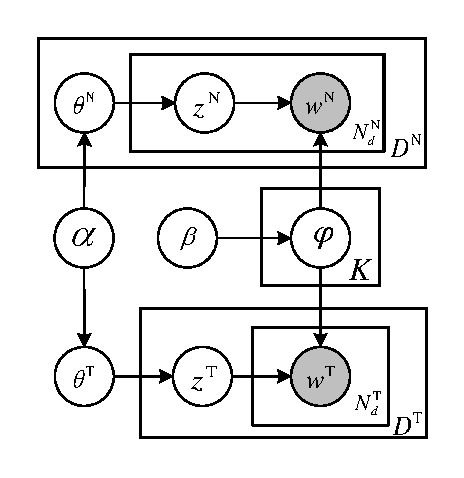
\includegraphics[width=.8\linewidth]{2016_icwsm_topicDynamic/figures/stlda_model.pdf}
\caption{Graphical Model of \stlda}\label{fig:stlda}
\end{figure}

The model's news part is the same as that of conventional LDA, but its tweet part is different. Specifically, the coverage of two plates are different, which is adapted according to our assumptions. The first difference is the coverage of word plate (the one with subscript $N^\mathrm{T}_d$). In LDA, it covers both $\bm{z}$ and $\bm{w}$, denoting that every word has its own topic assignment and every document consists of a mixture of topics. In \stlda's tweet part, the plate only covers $\bm{w}$, which means that every word in a tweet is generated from the same topic.

The second difference is the coverage of document plate (the one with subscript $D^\mathrm{T}$). LDA assumes that every document has a topic distribution, but in \stlda, every tweet only has one topic which can not form a distribution inside a document. Thus, $\bm{\theta^\mathrm{T}}$ is outside the document plate and denotes a background topic distribution of tweets. The posterior inference of \stlda is done by Gibbs sampling.

%\subsection{Posterior Inference}


%The sampling equation for news documents is the same as conventional LDA. The probability of $n$-th token in news document $d$ being assigned to a topic $k$ is computed as

%\begin{align}
%&\prob {z_{d,n}=k} {\bm{z_{-d}},\bm{w_{-d,n}},w_{d,n}=v} \notag\\
%\propto &\left( N_{d,k}^{-d,n} + \alpha \right) \frac {N_{k,v}^{-d,n} + \beta } {N_{k,\cdot}^{-d} + V\beta},
%\end{align}
%where $N_{d,k}$ denotes the number of tokens in document $d$ assigned to topic $k$; $N_{k,v}$ denotes the count of word $v$ assigned to topic $k$. Marginal counts are denoted by $\cdot$. $^{-d,n}$ denotes that the count excludes the $n$-th token in document $d$.

%The probability of tweet $d$ being assigned a topic $k$ is computed as

%\begin{align}
%&\prob {z_d=k} {\bm{z_{-d}},\bm{w}} \notag\\
%\propto &\left( N_k^{-d} + \alpha \right) \frac {\prod\limits_{v=1}^{V} \prod\limits_{i=0}^{N_{d,v}-1} \left( N_{k,v}^{-d} + \beta + i \right)} {\prod\limits_{i=0}^{N_{d,\cdot}-1} \left( N_{k,\cdot}^{-d} + V\beta + i \right)},
%\end{align}
%where $N_k$ denotes the number of documents assigned to topic $k$; $N_{d,v}$ is the count of word $v$ in document $d$. $^{-d}$ denotes that the count excludes document $d$.

%A brief derivation of Gibbs sampling equation is attached in %Appendix~\ref{sec:derivation}.

% After we train a model on training corpus, we can apply it on unseen documents and infer their topic assignments. The Gibbs sampling equation for test is much simpler. The probability of assigning topic $k$ to document $d$ is

% \begin{equation}
% \prob {z_d=k} {\bm{z_{-d}},\bm{w_d}} \propto \left( N_k^{-d} + \alpha \right) \prod_{v=1}^{V} \phi_{k,v}^{N_{d,v}}.
% \end{equation}

\subsection{Topic Dynamics}
The output results of \stlda model can be used for further discovery of topic dynamics of tweets and news. We define topic dynamics as temporal change of topics using daily sliding window. Assuming that every news document has the same impact and contributes equally to the total media environment, the topic proportion of day $t$ is the average of topic probabilities of all news documents on that day as

\begin{equation}
\bar{\theta}_{t,k}^{\mathrm{news}}=\frac{\sum_{d=1}^{D_t^{\mathrm{news}}} \theta_{d,k}}{D_t^{\mathrm{news}}},
\end{equation}
where $D_t^{\mathrm{news}}$ denotes the number of news documents on day $t$; $\theta_{d,k}$ is topic $k$'s proportion in document $d$.

Differently, each tweet $d$ has only one topic $z_d$ given by \stlda. Under the same assumption that each tweet contributes equally to the voice of public, the aggregation of daily tweet topic proportion is calculated as

\begin{equation}
\bar{\theta}_{t,k}^{\mathrm{tweets}} = \frac{\sum_{d=1}^{D_t^{\mathrm{tweets}}} \mathbbm{1}(z_d=k)}{D_t^{\mathrm{tweets}}},
\end{equation}
where $D_t^{\mathrm{tweets}}$ denotes the number of tweet documents on day $t$ and $\mathbbm{1}(\cdot)$ is an indicator function.

Given $\bm{\bar{\theta}_t^{\mathrm{news}}}$ and $\bm{\bar{\theta}_t^{\mathrm{tweets}}}$ where $t$ varies from August 11 to 27, we can identify topic dynamics by the changing of daily topic proportions. 